\documentclass[a4paper, 12pt]{article}
\usepackage{graphicx} % for including graphics
\usepackage{caption}  % for customizing figure captions

\makeatletter
\@addtoreset{figure}{section} % Reset figure numbering at the start of each section
\renewcommand{\thefigure}{\thesection.\arabic{figure}} % Format figure numbers as "1.1", "1.2", etc.
\makeatother

\renewcommand{\figurename}{Gambar} % Change "Figure" to "Gambar"

\begin{document}

\section*{DAFTAR GAMBAR}
\vspace{1em}
\renewcommand{\listfigurename}{List of Gambar} % Change "List of Figures" to "List of Gambar"
\listoffigures % Generates the list of figures

\section{Introduction}

In this section, we include the following figures:

% Gambar 1.1
\begin{figure}[h]
\centering
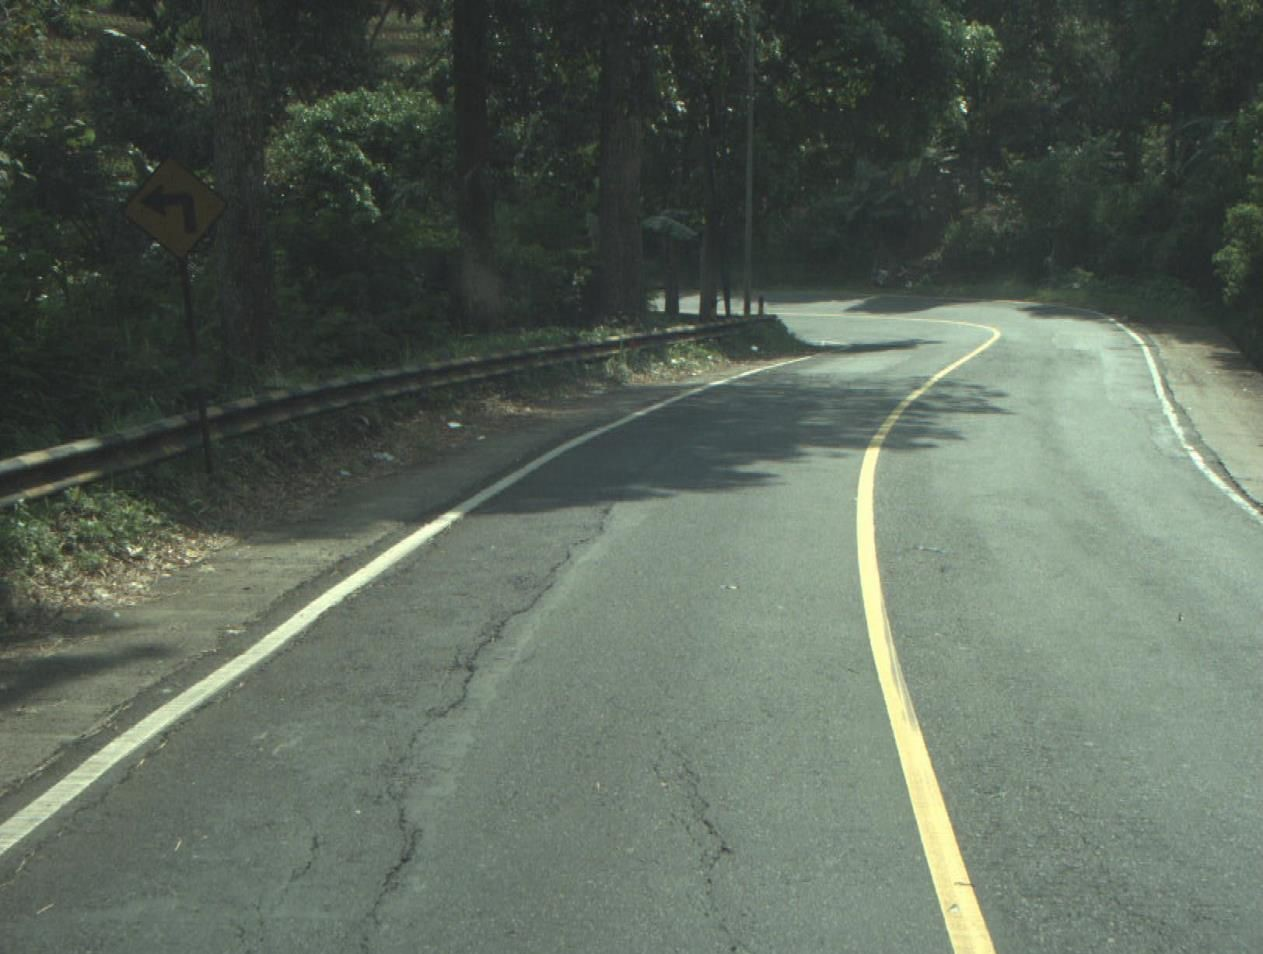
\includegraphics[width=0.3\textwidth]{figure1.jpeg}
\caption{Ini adalah Gambar 1.1.}
\label{fig:figure1}
\end{figure}

% Gambar 1.2
\begin{figure}[h]
\centering
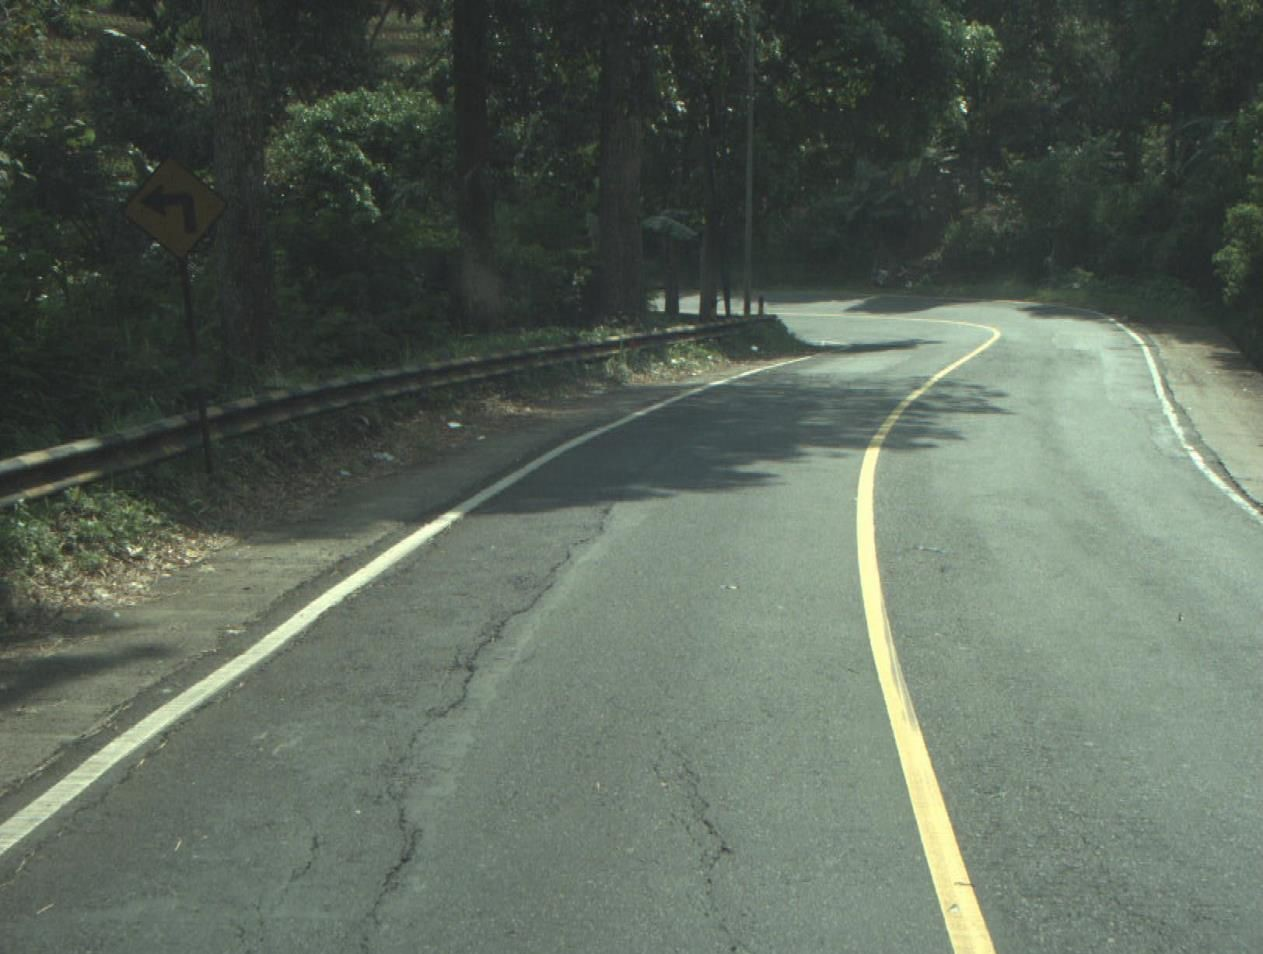
\includegraphics[width=0.3\textwidth]{figure1.jpeg}
\caption{Ini adalah Gambar 1.2.}
\label{fig:figure2}
\end{figure}

\section{Another Section}

In this section, we will have more figures:

% Gambar 2.1
\begin{figure}[h]
\centering
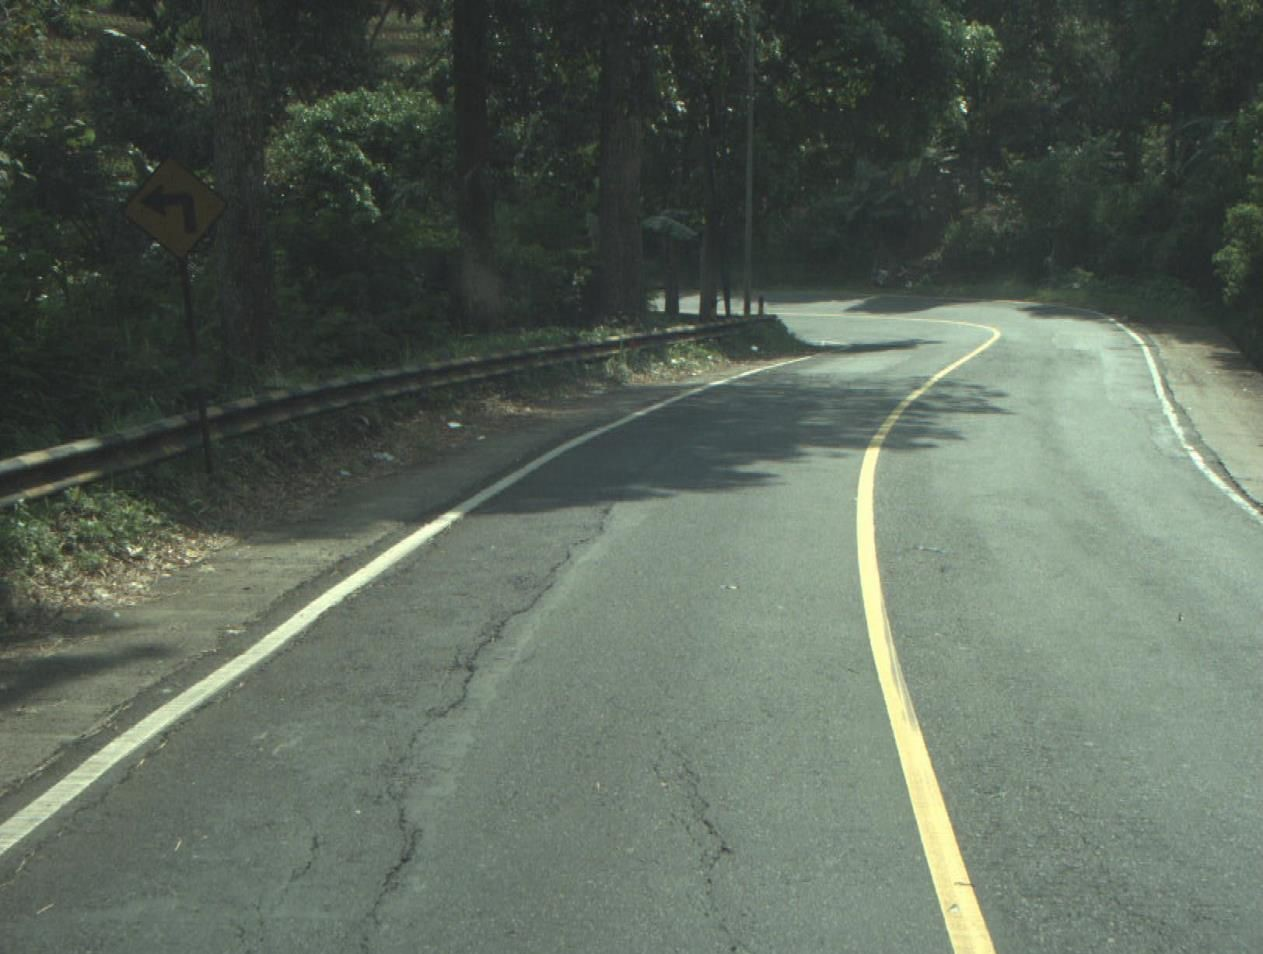
\includegraphics[width=0.3\textwidth]{figure1.jpeg}
\caption{Ini adalah Gambar 2.1.}
\label{fig:figure3}
\end{figure}

% Gambar 2.2
\begin{figure}[h]
\centering
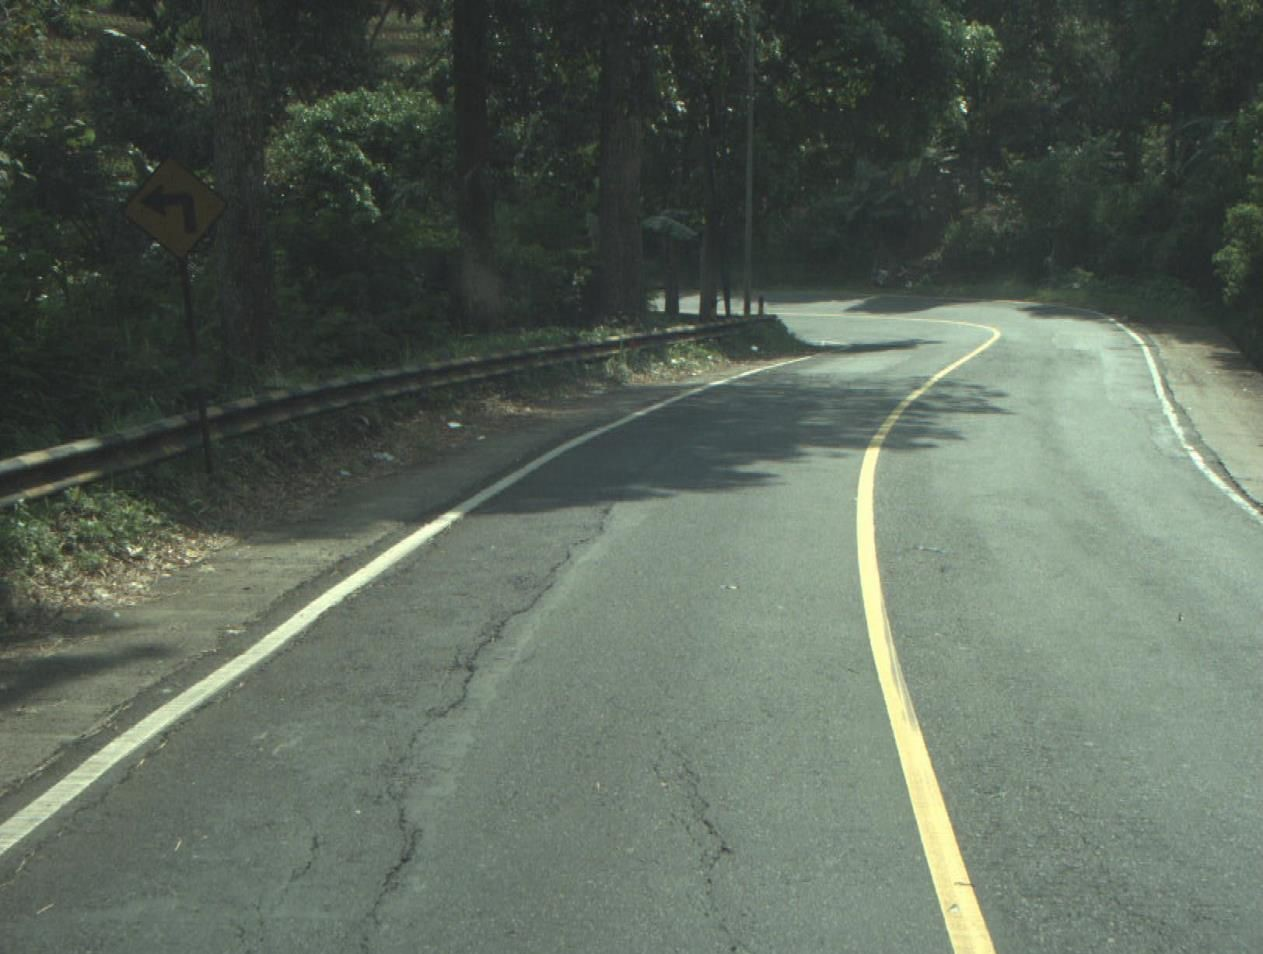
\includegraphics[width=0.3\textwidth]{figure1.jpeg}
\caption{Ini adalah Gambar 2.2.}
\label{fig:figure4}
\end{figure}

\end{document}
